\chapter*{Project Specification}
This project specification for the Master's Thesis has been accepted by Romain Claret (the student) and Jean Hennebert (the supervisor) on the 4th of October 2019 at HES-SO//Fribourg.

\section*{Introduction}
New technologies are revolutionizing the way humans access and consume information from multiple platforms and providers. Thanks to the emergence of increasingly powerful \gls{ai} algorithms, particularly in the field of \gls{nlp}, conversational agents, commonly known as chatbots, have come a long way and became popular among information consumers. As it is in late 2019, chatbots are all still \gls{ani}\footnote{The State of AI Report 2019 report by Nathan Benaich and Ian Hogar\cite{studies:state_of_ai_2019}}. Even if they are improving at providing meaningful sentences, they cannot generalize the tasks toward human-like conversations. Tasks such as understanding and keeping track of context in the long term, or even being intuitive and initiating meaningful conversation, have yet to be accomplished. Nonetheless, as research progress, chatbots are provided new tools which are making them step by step closer to complete human-like discussions, slowly progressing towards \gls{agi} chatbots.


\section*{Aim of the Study}
In harmony with the author's interest, the thesis' orientation goes toward research. Indeed, the study will attempt to explore approaches to get closer to general conversational agents as a premise to \gls{agi}. As a fulfillment of the academic requirements, the study will include an experimental part with one or many Proofs of Concept.

\subsection*{Project's Overall Scope}
The study is focusing on the English language as an attempt to increase the number of compatible datasets and make community accessible solutions. Complementarily, as the time for the thesis is limited to 19 weeks, the outcomes narrow at providing research conclusions and \gls{poc} solutions. We will be focusing at exploring two types of systems for \gls{qa} chatbots. The first type will produce straight to the point answers, and the second type will generate sentences as answers. Finally, the review of the risks and ethical problems that could be raised by the development of such solutions are not part of this work.
%\newpage


\subsection*{Industrial Interest}
\textit{iCoSys}, the Institut of Complex Systems at the University of Applied Sciences and Arts at Fribourg, Switzerland, is interested in the results of this study for their \textit{AI-News} project\footnote{\url{AINews.ch}}. Its goal is to provide a chatbot-based system as a tool to press readers, to help them narrow their interests and deliver the right information. This project is in collaboration with the \textit{Swiss Innovation Agency} from the Swiss Confederation, \textit{La Liberté}, the daily newspaper from Fribourg and \textit{Djebots}, a startup selling narrow chatbots.

\section*{Research Questions}
We articulate here a set of questions as a driver to our research work. From these questions are declined objectives, and from objectives are declined milestones framing the plan. We also hope to provide meaningful answers to these questions at the end of the thesis.
\begin{itemize}[noitemsep]
    \item What are the components to make \gls{qa} chatbots?
    \begin{itemize}[noitemsep]
        \item How to tune \gls{qa} chatbots to make them as human-like as possible?
        \item How to tune such systems for the field of journalism?
    \end{itemize}
    \item What is the state of the art for generative \gls{qa} chatbots?
    \begin{itemize}[noitemsep]
    	\item What are the components to make make generative \gls{qa} chatbots?
        \item Are generative chatbots only as good as the data they consume?
        \item Could generative chatbots be a step toward \gls{agi}?
    \end{itemize}
\end{itemize}

\section*{Objectives}
\subsection*{Intrinsic}
This subsection presents the general objectives related to the master's thesis.
\paragraph{Primaries}
\begin{itemize}[noitemsep]
    \item Suggest project specification and planning.
    \item Analyze the state of the art of existing technologies and technics of \gls{qa} systems and generative \gls{ai}.
    \item Overview digital transformation in journalism and review the current status of the AI-News project.
    \item Document the study and write the thesis.
\end{itemize}

\subsection*{Fact-based \gls{qa} Chatbot}
The first objective is to make a state of the art software that takes a question as input and outputs a response (See Figure \ref{fig:spec_qa}).
\begin{figure}[ht!]
    \centering
    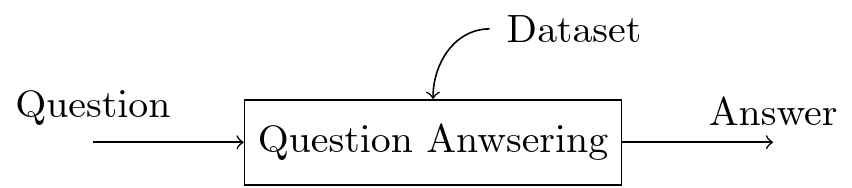
\includegraphics[width=\textwidth,height=2.2cm,keepaspectratio=true]{intro_qa}
    \caption{Suggested \gls{qa} diagram}
    \label{fig:spec_qa}
\end{figure}

\paragraph{Primaries}
\begin{itemize}[noitemsep]
    \item Select existing papers and projects treating the subject as a starting point.
    \item Identify relevant datasets.
    \item Develop one or more \gls{poc}.
    \item Test and evaluate solutions.
    \item Suggest improvements, possible continuation, and future outcomes.
\end{itemize}
\paragraph{Secondaries}
\begin{itemize}[noitemsep]
    \item Extended the \gls{qa} chatbot using tailored knowledge.
\end{itemize}

\subsection*{Generative \gls{qa} Chatbot}
The second objective is to improve the output from the prior objective into enhanced answers (See Figure \ref{fig:spec_qa_gen}).
\begin{figure}[ht!]
    \centering
    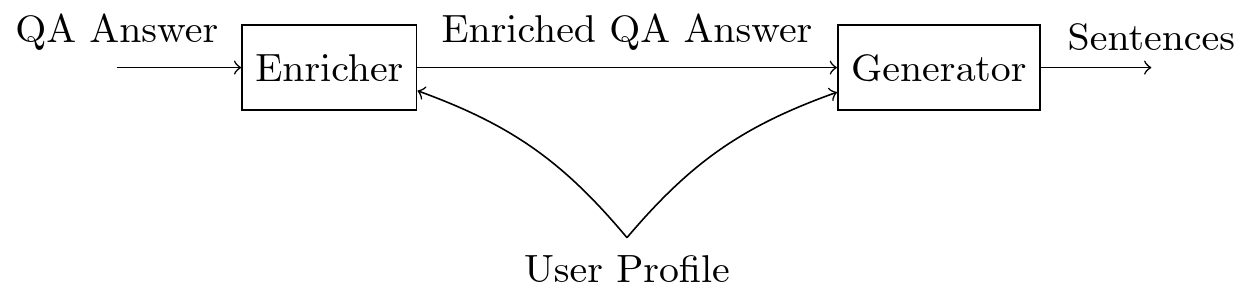
\includegraphics[width=\textwidth,height=6cm,keepaspectratio=true]{intro_qa_gen}
    \caption{Suggested Generative \gls{qa} diagram}
    \label{fig:spec_qa_gen}
\end{figure}

\paragraph{Primaries}
\begin{itemize}[noitemsep]
    \item Investigate a rule-based system for keyword enrichment.
    \item Generate sentences with keywords.
    \item Identify relevant datasets.
    \item Develop one or more \gls{poc}.
    \item Test and evaluate solutions.
    \item Suggest improvements, possible continuation, and future outcomes.
\end{itemize}
\paragraph{Secondaries}
\begin{itemize}[noitemsep]
    \item Use advanced strategies to enrich keywords.
    \item Use advanced text generation technics such as GTP-2\footnote{OpenAI's GTP-2 Algorithm\cite{papers:gpt2}}.
    \item Use user profiles to customize the outputs.
\end{itemize}


\section*{Plan}
\label{plan:plan}
\subsection*{Contraints}
\textbf{Timeframe:} 19 weeks\\
\textbf{Starting date:} 16.09.2019\\
\textbf{Ending date:} 07.02.2020

\subsection*{Methodologies}
For consistency, the project is split into two methodological parts. The first third, as the project's orientation is going toward information gathering and self-study, uses a standard sequential project management methodology. For the next two-thirds of the project, the author is using an agile methodology intending to reach incremental progress while exploring.

\subsubsection*{Back to level Milestones}
\textbf{(6 weeks)} First third of the study, from \textbf{16.09.19 to 25.10.19}.
\begin{enumerate}
    \setlength\itemsep{0em}
    \item[M1.] Initial \gls{mt} plan and project specification
    \item[M2.] Review the state of the art of the \gls{nlp} and \gls{nlu} technologies and refine the plan if needed.
\end{enumerate}


\subsubsection*{Diving into the subject Milestones}
\textbf{(13 weeks) From 28.10.19 to 07.02.20}, the following two-third of the thesis is composed 6 of sprints of two weeks and one week to finalise the thesis.
\begin{itemize}
    \setlength\itemsep{0em}
    \item[M3.] Basic \gls{qa} Chatbot
    \item[M4.] Evaluation of basic \gls{qa} Chatbot
    \item[M5.] Basic generative \gls{qa} Chatbot
    \item[M6.] Evaluation of basic generative \gls{qa} Chatbot
\end{itemize}

\subsection*{Gantt}
The Figure~\ref{fig:gantt-specification} represents the chart for the initial plan.

\newganttchartelement*{specifications-milestones}{
specifications-milestones/.style={
shape=isosceles triangle,
inner sep=0pt,
draw=cyan,
top color=white,
bottom color=cyan!50
},
specifications-milestones incomplete/.style={
/pgfgantt/specifications-milestones,
draw=yellow,
bottom color=yellow!50
},
specifications-milestones label font=\slshape,
specifications-milestones left shift=0pt,
specifications-milestones right shift=0pt
}

\newgantttimeslotformat{stardate}{
\def\decomposestardate##1.##2\relax{
\def\stardateyear{##1}\def\stardateday{##2}
}
\decomposestardate#1\relax
\pgfcalendardatetojulian{\stardateyear-01-01}{#2}
\advance#2 by-1\relax
\advance#2 by\stardateday\relax
}

\begin{figure}[h]%[htbp]
\centering
\begin{ganttchart}[vgrid, hgrid]{1}{19}
\gantttitle{Sep}{2} 
\gantttitle{Oct}{5}
\gantttitle{Nov}{4}
\gantttitle{Dec}{3}
\gantttitle{Jan}{4}
\gantttitle{Feb}{1}\\
\gantttitlelist{1,...,19}{1}\\

%part 1
\ganttgroup{Back to level}{1}{6} \\
\ganttmilestone{M1, M2}{3}
\ganttmilestone{}{6}\\

%part 2
\ganttgroup{Diving}{7}{18} \\
\ganttbar{Sprint 1}{7}{8} \\
\ganttbar{Sprint 2}{9}{10} \\
\ganttmilestone{M3}{10}\\
\ganttbar{Sprint 3}{11}{12} \\
\ganttmilestone{M4}{12}\\
\ganttbar{Sprint 4}{13}{14} \\
\ganttbar{Sprint 5}{15}{16} \\
\ganttmilestone{M5}{16}\\
\ganttbar{Sprint 6}{17}{18} \\
\ganttmilestone{M6}{18}\\

%\ganttlink{elem6}{elem7}
%\ganttlink{elem8}{elem9}

%part 3
\ganttgroup{Wrap up}{19}{19} \\


\end{ganttchart}

\caption{Project Specificiation Gantt Chart}
\label{fig:gantt-specification}
\end{figure}
